\chapter{FOOT DEFORMITIES}\label{chp:Feet Deformities}

Correspondingly, this chapter gives an overview of significant and relevant research in pes planus and pes cavus medical treatments and detection methods.

\section{PES PLANUS AND PES CAVUS}

Abnormalities and irregularities in the normal structure of the medial longitudinal arch cause functionally unstable conditions of the foot such as pes cavus or pes planus. Pes planus is the loss of the medial longitudinal arch of the foot that results in the entire bottom of the foot approaching or touching the ground while walking or standing \cite{wozniacka2013body} (see Figure \ref{fig:BackgroundPesPlanus}). This arch acts as a flexible and adaptable foundation for the entire body \cite{kohls2009prevalence}, and its functionality is also vital to the body as it relieves the stresses of weight-bearing during the walking cycle and stores mechanical energy within the stretched elastic ligaments \cite{da1963idiopathic}. Although it may be asymptomatic, a defective medial longitudinal arch can alter the biomechanics of the lower extremities and lumbar spine, resulting in an increased risk of pain and injury \cite{gun2012pes}.

\begin{figure}[htbp]
\centering
\fbox{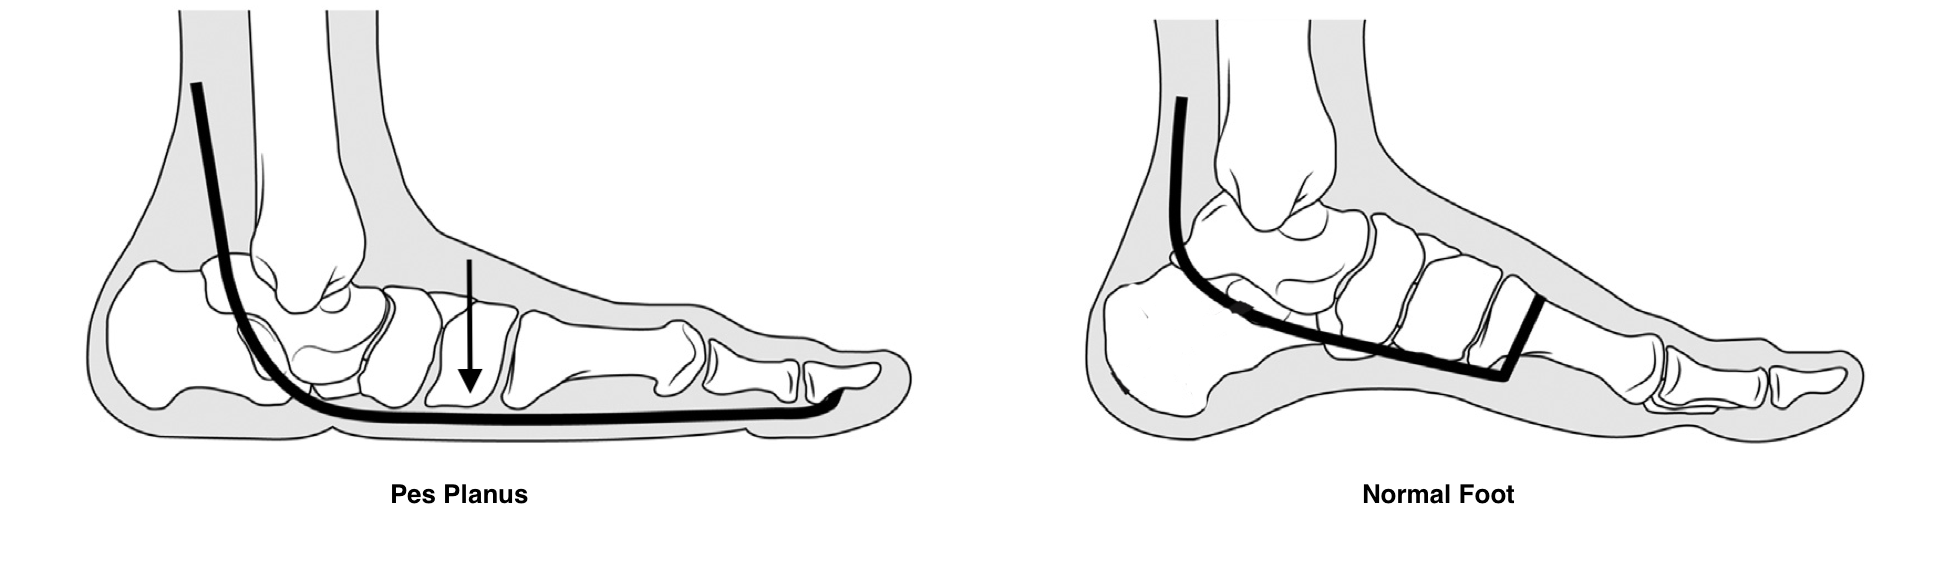
\includegraphics[width=.8\columnwidth]{KaanEksenMSc/figures/BackgroundPesPlanus.png}}
\caption{Pes planus \cite{kim2021dynamic}}
\label{fig:BackgroundPesPlanus}
\end{figure}

Pes planus is caused by a variety of reasons that might be acquired or congenital. By the age of six, the majority of congenital pes planus abnormalities have vanished, and this is a normal aspect of human body development \cite{Mickle2006TheFO}. However, some congenital conditions can persist throughout adulthood, particularly those associated with obesity \cite{Woniacka2013BodyWA}. Pes planus can, however, develop as a result of various malformations in the extremities. One of the most prevalent causes of pes planus is functional issues with the posterior tibial tendon, which sustains the arch of the foot and allows for inversion and plantarflexion. Females over forty who have diabetes or are overweight are more likely to have posterior tibial tendon damage \cite{KohlsGatzoulis2009ThePO}. In addition, pes planus can be developed more commonly in patients with congenital ligamentous laxity secondary to Down syndrome, Ehlers Danos or Marfan. Pes planus is also common among patients who have had midfoot or hindfoot trauma, such as a navicular, first metatarsal, or calcaneal fracture, or a Lisfranc ligament complex injury.

\begin{figure}[htbp]
\centering
\fbox{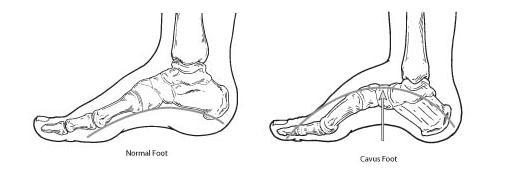
\includegraphics[width=.8\columnwidth]{KaanEksenMSc/figures/BackgroundPesCavus.jpg}}
\caption{Pes planus \cite{physiopediapescavus}}
\label{fig:BackgroundPesCavus}
\end{figure}

Pes cavus,  on the other side, is foot deformity distinguished by an elevation of the plantar longitudinal arch (see Figure \ref{fig:BackgroundPesCavus}). Clawing of the toes, posterior hindfoot deformity, plantar fascia contracture, and defects in the great toe are all common deformities associated with pes cavus. Furthermore, a common symptom of an underlying neurological disorder is pes cavus \cite{Brewerton1963IDIOPATHICPC}.

\section{MEDICAL DETECTION SOLUTIONS}

Pes planus and pes cavus have been diagnosed using ultrasonographic reviews, radiological evaluation, somatometric measurement, and clinical examination. In addition, indirect (or non-anthropometric) measurements are also utilized in the literature to detect pes planus and pes cavus, such as Inked or digital footprints (pressure measurements) and photographic \cite{gun2012pes, yalccin2010medial}. However, radiological evaluations \cite{Smith1997PrevalenceOR, Winfeld2019ManagementOP} are the most well-accepted and used approach for detecting pes planus and pes cavus in a wide range of solutions.

Chung et al. \cite{Chen2010FootprintAO} used the well-accepted radiographic detection technique to evaluate radiological data of 103 subjects' navicular and talar heights and the arch index. According to their findings, the Staheli arch index, Chippaux-Smirak index, and Clarke's angle have 85.43 percent, 90.54 percent, and 83.89 percent prediction probability in preschool-aged children correspondingly. In another research, Pauk et al. \cite{Pauk2014AssessingPP} evaluate Clarke angle and radiography data of sixty kids. Correlation between radiography and the footprints discovered in the research. Correspondingly, many research have been conducted to examine the relationship between footprint and radiography methodologies \cite{Kanatl2001FootprintAR, Yaln2010EvaluationOT, menz2005validity}.

Aside from the comparisons research presented above, several studies in the literature only use non-anthropometric methods to detect pes planus or pes cavus, such as planimeter \cite{Didia1987TheUO} or arch index \cite{Cavanagh1987TheAI, Igbigbi2002TheFR}. Aside from the comparisons research presented above, several studies in the literature only use non-anthropometric methods to detect pes planus or pes cavus, such as planimeter \cite{Didia1987TheUO} or arch index \cite{Cavanagh1987TheAI, Igbigbi2002TheFR}. Consequently, the non-anthropometric methods' applicability has been demonstrated to be viable.

On 305 Maldivians between the ages of 13 and 17, Igbigbi et al. \cite{Igbigbi2002TheFR} used an arch index (footprint ratio) to identify arc type and pes planus ratio. Subjects' foot data is obtained in this study by making an imprint of the participant's sole with ink and a piece of paper. According to the authors, the technique employed is cost-effective, resilient, and more efficient.

However, Kanatli et al. \cite{Kanatl2001FootprintAR} used 38 pre-schoolers and school-aged children with an average age of 6.4 (ages range from 3.7–11.7) to compare radiologic measures and footprint methodologies in order to determine the association between the two approaches. According to the data, there is a strong link between arch index, talo–horizontal angle, and talo-first metatarsal angle. On the other side, they discovered no link between arch index, lateral talocalcaneal angles, and calcaneal pitch.

A study that compared footprint and radiographic measures on 338 people found a decent association between the Staheli index, the Grivas Classification System, and the Chippaux-Smirak index with a similar impression \cite{gun2012correlation}. The authors emphasize, however, that there is a limited association between the radiological measurement methods calcaneal pitch angles and talo-first metatarsal angle and all three footprint measurement methods as a result of the findings. However, the authors highlight a limited association between the radiological measurement methods, the talo-first metatarsal angle and calcaneal pitch angles, and all three footprint measurement methods as a result of the findings. Furthermore, the findings show that the footprint measurement methods and talo-horizontal angle have no meaningful correlation.

\section{PES PLANUS AND PES CAVUS DETECTION TOOLS}

There are a variety of produced systems for detecting foot abnormalities, ranging from simple solutions like planimeter \cite{Didia1987TheUO} to far more advanced systems like gait analysis \cite{Buldt2015FootPI}.

Gait analysis \cite{sennotech_2021,alfoots_2021} is used by the majority of commercially available devices to detect a variety of foot abnormalities. Optical motion capture systems (OMCS) \cite{vicon_2021} are also used by some of these systems to detect foot abnormalities. Nevertheless, having this extra equipment for greater accuracy increases the required budget.

Moreover, some businesses like Sennotech's Senno Gait are designing low-cost solutions to address the market gap by reducing sensitivity. For example, Sennotech \cite{sennotech_2021} analyzes gait using low-cost sensors and AI models. As a result, these devices are less expensive and easier to use, and they provide information such as injury concerns and irregular movement.

\begin{figure}[htbp]
\centering
\fbox{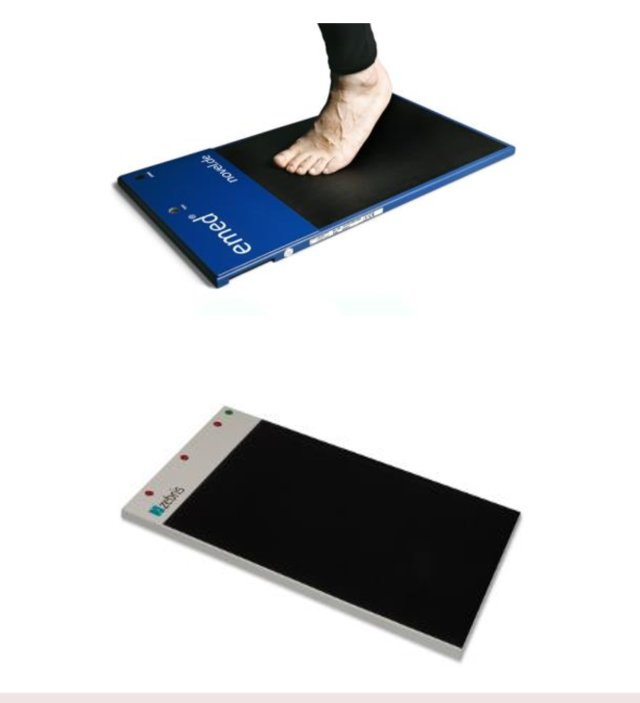
\includegraphics[width=.4\columnwidth]{KaanEksenMSc/figures/BackgroundExampleEmed.jpg}}
\caption{EMED \cite{articleFootPressure}}
\label{fig:BackgroundExampleEmed}
\end{figure}

Many researchers \cite{Buldt2018FootPI, articleKeukenkampDiabeticMedicine, BOSCH2010564} have employed pressure detection devices \cite{novel_2021, medilogic_2021}. These devices are far more widely available than OMCS equipment. However, they provide fewer data. Buldt et al. \cite{Buldt2018FootPI}, for example, employed EMED, a pressure sensing device, to assess pes planus and pes cavus in their research.